\section{3D Rendering Grundlagen}
In den weiterführenden Abschnitten werden Kenntnisse über grundlegende Begriffe und Konzepte des 3D Renderings benötigt.
Deshalb werden diese in diesem Abschnitt erklärt.
Die benötigten Themen wurden in WebGL: up and running \cite[4-9]{parisi2012webgl} passend zu den folgenden Kapiteln gegliedert, deshalb wurde die Struktur dieser Grundlagen an diese angelehnt.

\subsection{3D Koordinatensystem}
Beim Rendern von 2D Elementen wird ein einfaches 2D Koordinatensystem verwendet, genauso wie man es aus der Mathematik kennt. Dort gibt es eine x- und eine y-Achse, durch welche die Koordinaten der einzelnen Punkte beschrieben werden können.
Dabei ist es üblich, dass die x-Achse horizontal liegt und somit bestimmt wie weit Links oder Rechts der Punkt ist. Die y-Achse hingegen bestimmt wie hoch und tief ein Punkt liegt.
Um nun zum 3D Koordinatensystem zu kommen, wird einfach eine dritte Achse hinzugefügt, die z-Achse. Diese steht beim WebGL Koordinatensystem so gesehen aus dem Bildschirm heraus, das heißt,
 negative Werte geben an wie tief ein Punkt im Bildschirm liegt. \cite[4]{parisi2012webgl} In Abbildung~\ref{fig:3DKoordinatensystem} sieht man exemplarisch ein solches 3D Koordinatensystem.
 \begin{figure}
    \centering
    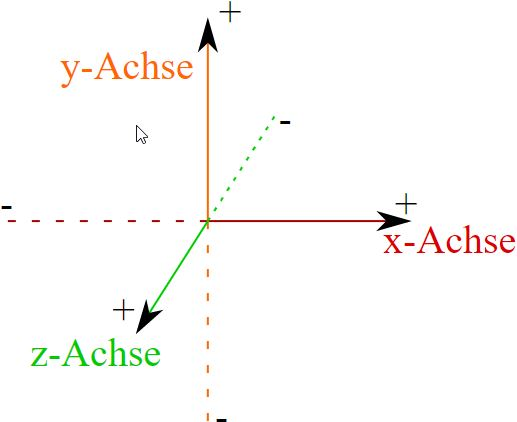
\includegraphics[width=6cm]{3dkoords.jpg}
    \caption{3D Koordinatensystem \cite{PeterStrohm}} \label{fig:3DKoordinatensystem}
    \end{figure}

\subsection{Gittergewebe, Polygone und Eckpunkte}
Es gibt sehr viele verschiedene Arten 3D Grafiken zu zeichnen, am meisten werden dafür so genannte Gittergewebe auch bekannt als Meshes verwendet.
Ein solches Mesh besteht aus einem oder mehreren Polygonen Formen, meist Dreiecke oder Vierecke. Definiert sind diese Drei- und Vierecke durch drei bzw.
vier Vektoren wobei jeder Vektor für einen Punkt im 3D Koordinatensystem steht also x, y und z.
Ein 3D Mesh wird oft auch als Model bezeichnet, ein Beispiel hierfür ist in Abbildung~\ref{fig:Mesh} zu sehen. \cite[4]{parisi2012webgl}
\begin{figure}
    \centering
    \includegraphics[width=6cm]{Meshes.jpg}
    \caption{Wireframe von einem Mesh \cite{sketchfab}} \label{fig:Mesh}
    \end{figure}

\subsection{Materialien, Texturen und Lichter}
Um nun die Oberfläche eines Meshes zu beschreiben, bedarf es mehr als nur den verschiedenen Vektoren.
Auch hier gibt es verschiedene Arten die Oberfläche zu beschreiben, die einfachste wäre der Oberfläche einfach eine Farbe zuzuweisen.
Möchte man die Oberflächen nun genauer beschreiben bedarf es deutlich mehr Informationen, zum Beispiel wie Lichter von der Oberfläche reflektiert werden sollen oder ob die Oberfläche leuchten soll und so weiter.
Außerdem kann man, anstatt nur eine Farbe zu definieren auch so genannte Texturen verwenden, dies sind meist Bitmaps, welche beschreiben wie ein kleines Stück einer bestimmten Oberfläche aussieht.
Dieses Stück ist meist so gegeben das es endlos aneinandergehängt werden kann und somit eine beliebig große Fläche füllen kann.
In vielen Bild- und Videobearbeitungsprogrammen werden alle Eigenschaften einer Oberfläche zusammen als Materialien bezeichnet.
Da viele Eigenschaften eines Material erst bei Auftreffen von Licht zum Vorschein kommen, benötigen viele Materialien Licht umso auszusehen wie gewollt. \cite[5]{parisi2012webgl} 
%evtl Beispieltextur einfügen und darauf eingehen

\subsection{Transformationen und Matrizen}
Bei vielen 3D Anwendungen möchte man nun ein Model auch bewegen oder sogar animieren können, dafür gibt in den meisten Programmen Transformationen.
Diese sorgen dafür das man ein ganzes Model als eines bewegen, drehen oder skalieren kann und nicht jedes einzelne Eck nacheinander bewegen muss.
Diese Transformationen werden durch Matrizen beschrieben, das heißt, um eine Drehung zu erhalten wird einfach durch lineare Algebra aus der Matrix und dem Model die neuen Positionen des Models berechnet. \cite[6,7]{parisi2012webgl}

\subsection{Kameras, Perspektiven, Ansichtsfenster und Projektionen}
Um eine 3D Szene zu rendern benötigt man eine Perspektive, aus der auf die Szene geschaut wird.
Die meisten 3D Programme verwenden hierfür Kameras, diese können wie ein eigenes Objekt platziert und transformiert werden.
Auch hier werden Matrizen verwendet, eine besondere Matrix ist hier die Projektionsmatrix, welche dafür sorgt, dass aus der 3D Szene ein 2D Bild wird.
Hierbei ist das 2D Bild ein bestimmtes Ansichtsfenster der 3D Szene.
Sowohl hier als auch bei den Transformationen benötigt man als Nutzer der Programme meist keine Kenntnisse über lineare Algebra, sondern kann einfach per Drag und Drop eingestellt werden. \cite[7]{parisi2012webgl}
% evtl beispiel für kamera szene etc.

\subsection{Shader}
Als letztes gibt es noch Shader, diese definieren wie all die definierten Objekte, Kameras und Lichter miteinander interagieren.
Ein Shader ist ein kleines Programm, welches definiert wie alle Pixel der Meshes am Ende im Bild aussehen sollen.
Shader sind darauf ausgelegt von einer \ac{GPU} ausgeführt zu werden.
Bei anderen Grafikbibliotheken sind Shader optional, bei WebGL jedoch werden immer Shader benötigt und daher eine \ac{GPU} erwartet.
Auch hier gibt es jedoch einige Erleichterungen, die meisten WebGL Bibliotheken haben Standard Shader welche für die meisten Anwendungsfälle mehr als ausreichend sind. \cite[7-9]{parisi2012webgl}